% Digital Logic Report Template
% Created: 2020-01-10, John Miller

%==========================================================
%=========== Document Setup  ==============================

% Formatting defined by class file
\documentclass[11pt]{article}

% ---- Document formatting ----
\usepackage[margin=1in]{geometry}	% Narrower margins
\usepackage{booktabs}				% Nice formatting of tables
\usepackage{graphicx}				% Ability to include graphics

%\setlength\parindent{0pt}	% Do not indent first line of paragraphs 
\usepackage[parfill]{parskip}		% Line space b/w paragraphs
%	parfill option prevents last line of pgrph from being fully justified

% Parskip package adds too much space around titles, fix with this
\RequirePackage{titlesec}
\titlespacing\section{0pt}{8pt plus 4pt minus 2pt}{3pt plus 2pt minus 2pt}
\titlespacing\subsection{0pt}{4pt plus 4pt minus 2pt}{-2pt plus 2pt minus 2pt}
\titlespacing\subsubsection{0pt}{2pt plus 4pt minus 2pt}{-6pt plus 2pt minus 2pt}

% ---- Hyperlinks ----
\usepackage[colorlinks=true,urlcolor=blue]{hyperref}	% For URL's. Automatically links internal references.

% ---- Code listings ----
\usepackage{listings} 					% Nice code layout and inclusion
\usepackage[usenames,dvipsnames]{xcolor}	% Colors (needs to be defined before using colors)

% Define custom colors for listings
\definecolor{listinggray}{gray}{0.98}		% Listings background color
\definecolor{rulegray}{gray}{0.7}			% Listings rule/frame color

% Style for Verilog
\lstdefinestyle{Verilog}{
	language=Verilog,					% Verilog
	backgroundcolor=\color{listinggray},	% light gray background
	rulecolor=\color{blue}, 			% blue frame lines
	frame=tb,							% lines above & below
	linewidth=\columnwidth, 			% set line width
	basicstyle=\small\ttfamily,	% basic font style that is used for the code	
	breaklines=true, 					% allow breaking across columns/pages
	tabsize=3,							% set tab size
	commentstyle=\color{gray},	% comments in italic 
	stringstyle=\upshape,				% strings are printed in normal font
	showspaces=false,					% don't underscore spaces
}

% How to use: \Verilog[listing_options]{file}
\newcommand{\Verilog}[2][]{%
	\lstinputlisting[style=Verilog,#1]{#2}
}

\usepackage[section]{placeins}


%======================================================
%=========== Body  ====================================
\begin{document}


\title{ELC 2137 Lab 11: FSM: Guessing Game}
\author{Aaron Mendoza}

\maketitle


\section*{Summary}

The purpose of this lab is to build a guessing game in which the user presses buttons on a Basys3 board that correspond to certain states in order to win. 

The first module built during this lab was the debounce module. Although pressing a button is seemingly straightforward, there is actually something called a "bounce" where the output cycles on and off a few times when the button is pressed or a switch is moved. In order to fix this, I built a debounce module, where it changes between four states: zero, wait1, one, wait0. In order to switch from zero to one, the output from zero must remain on for a long enough time during wait1, in which case it will switch to one. If the output from zero does not remain on long enough during wait1, then it returns back to zero. This eliminates the bounce behavior from pressing the pushbuttons on the Basys3 board. This module has three inputs (in, reset, clock) and two outputs (out and tick). Tick corresponds with if the button was pressed, and out corresponds with how long the button was pressed.

The second module built during this lab was the guess-FSM module. This module contains the main states of the game. The guess-FSM module has six states: s0, s1, s2, s3, swin, and slose. Whenever there is no input given, the FSM cycles through s0 to s3. When there is an input given at one of those states, it will either go to swin or slose based on logic. My guess-FSM module has three inputs (clock, enable, and b) and three outputs (y, win, and lose). 

The third module built was just a counter module built from a previous lab. This controls the time it takes to switch between the states of my guess-FSM module. In other words, this controls the difficulty of the game. This is made possible by using a mux, where turning a switch on and off changes which counter is used. The only difference between the counters is the parameter N (number of bits) given within the code.  

My top level module guessing-game combines all of these previous modules. Each of the buttons on the Basys3 board(btnU, btnL, btnR, and btnD) feed into the input of a debounce module whose outputs go into the "b" input of the my guess-FSM module. The output of the mux whose inputs are from the counters are decided by sw[0] of the board, which goes into the enable input of my guess-FSM to keep the states switching from s0 to s3 at a constant rate. Finally, I made my y output of the guess-FSM module correspond with the states. In order to do this, I made a case statement where the y switches between the top four segments of the right most anode. In other words, the moving target is a dash that moves in a box on the display. This makes it easier for the user to pick the button that matches with the moving target. 


\section*{Q\&A}

\begin{enumerate}
	\item At what time in the simulation the did debounce circuit reach each of the four states (\verb||\textit{zero, wait1, one, wait0})?
	
		The debounce circuit reached zero at 20 ns, wait1 at 200 ns, one at 245 ns, and wait0 at 600 ns.

	\item Why can this game not be implemented with regular sequential logic?
	
		This game cannot be built using regular sequential logic because the outputs do not repeat or exhibit a specific pattern. So, in this lab I implemented a finite state machine. An FSM has a limited number of internal "states" that switch between each other based on the inputs. This is crucial for the game; the states are not just repeating from s0 to s1 to s2 to s3 all the time. Instead, s0 can go to swin, slose, or s1 based on the input, so an FSM is needed in order for this game to work.

	\item What types of outputs did you use for your design (Mealy or Moore)? Explain.
	
		Moore because it is safer than Mealy. This is the safer design because there is less risk for glitches. The output is only dependent on the current state, and if the inputs change the output changes as well. Although Mealy is faster, it is harder to design and puts me more at risk for glitches, so I used Moore.

\end{enumerate}


\section*{Results}

\begin{figure}[ht]\centering
	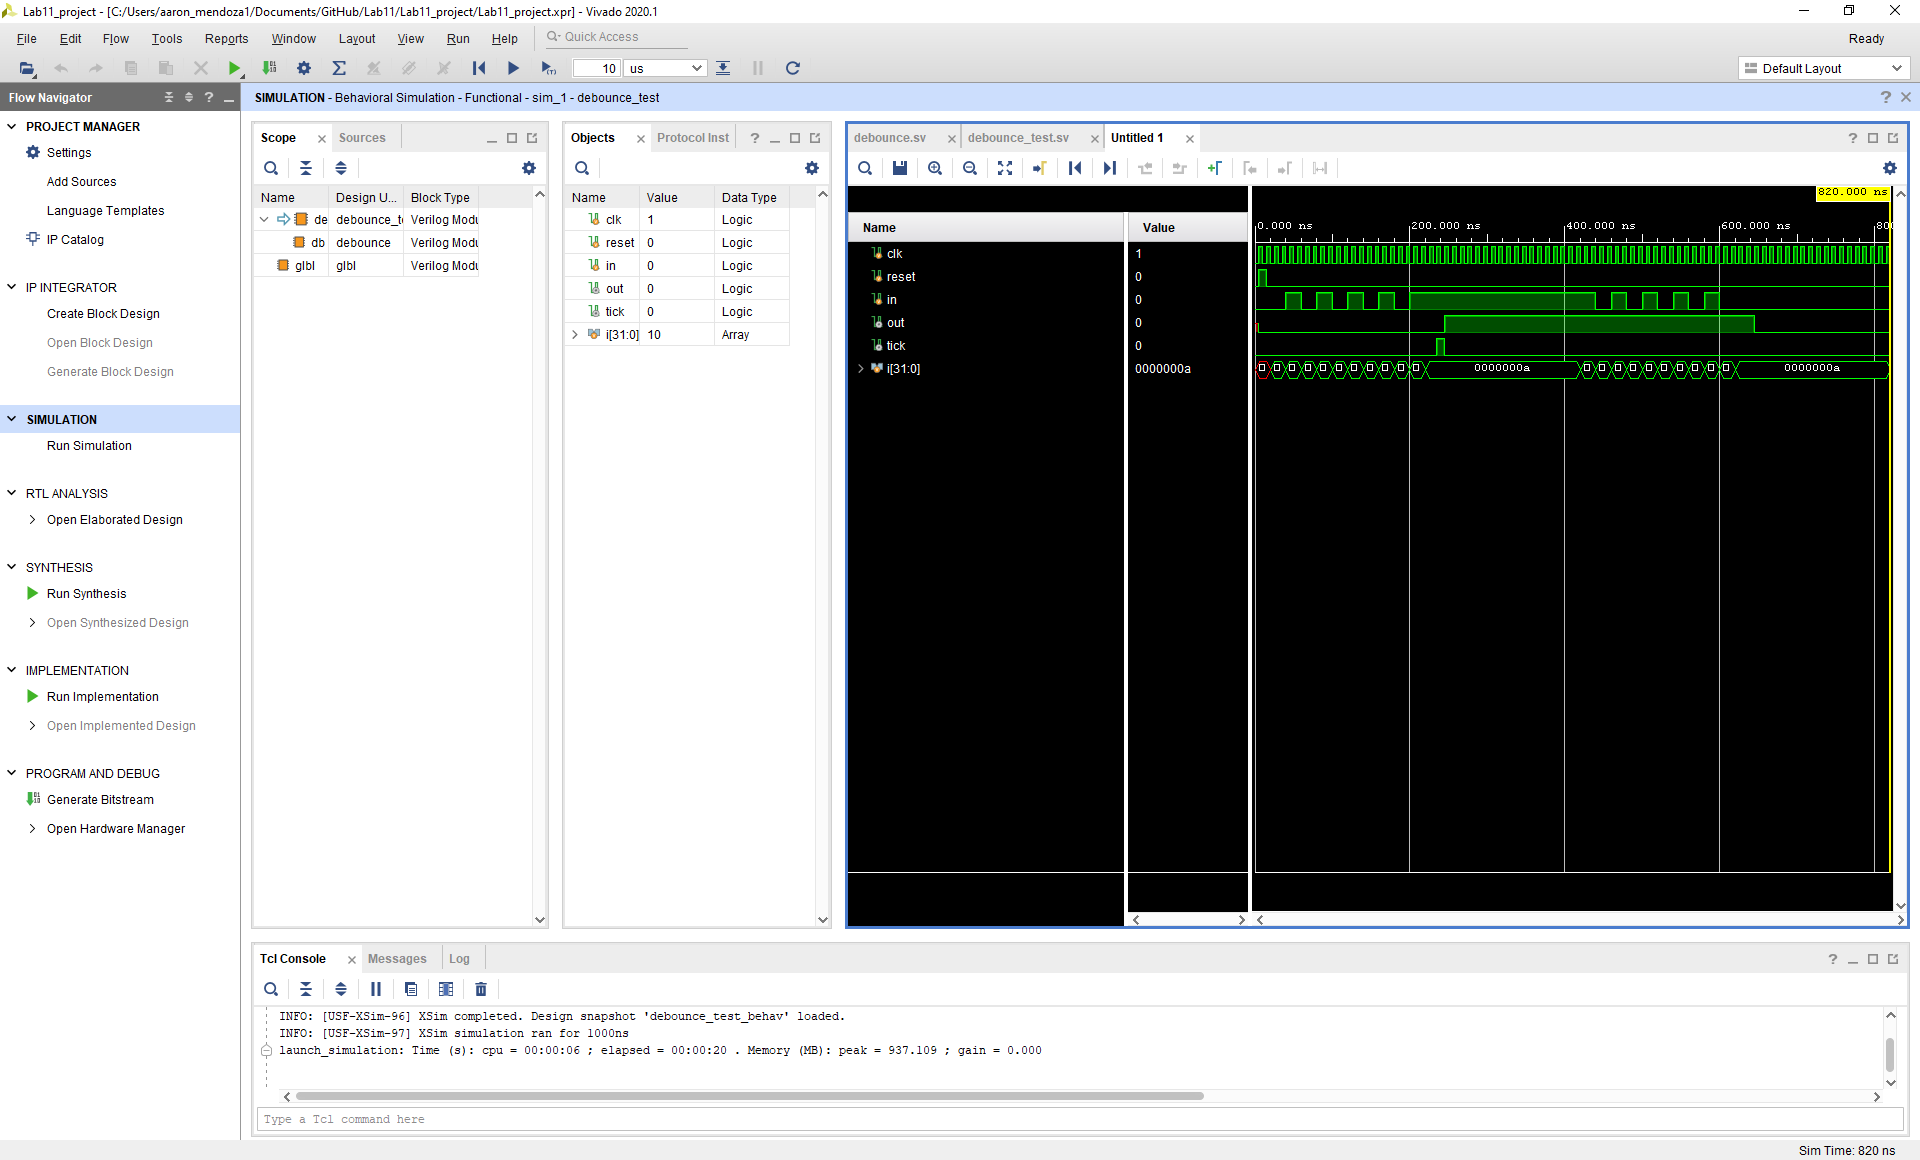
\includegraphics[width=1\textwidth,trim=32cm 20cm 0cm 4.5cm,clip]{debounce_test_screenshot}
	\caption{Debounce Simulation Screenshot}
	\label{fig:sim_with_table}
\end{figure}

\FloatBarrier

\begin{figure}[ht]\centering
	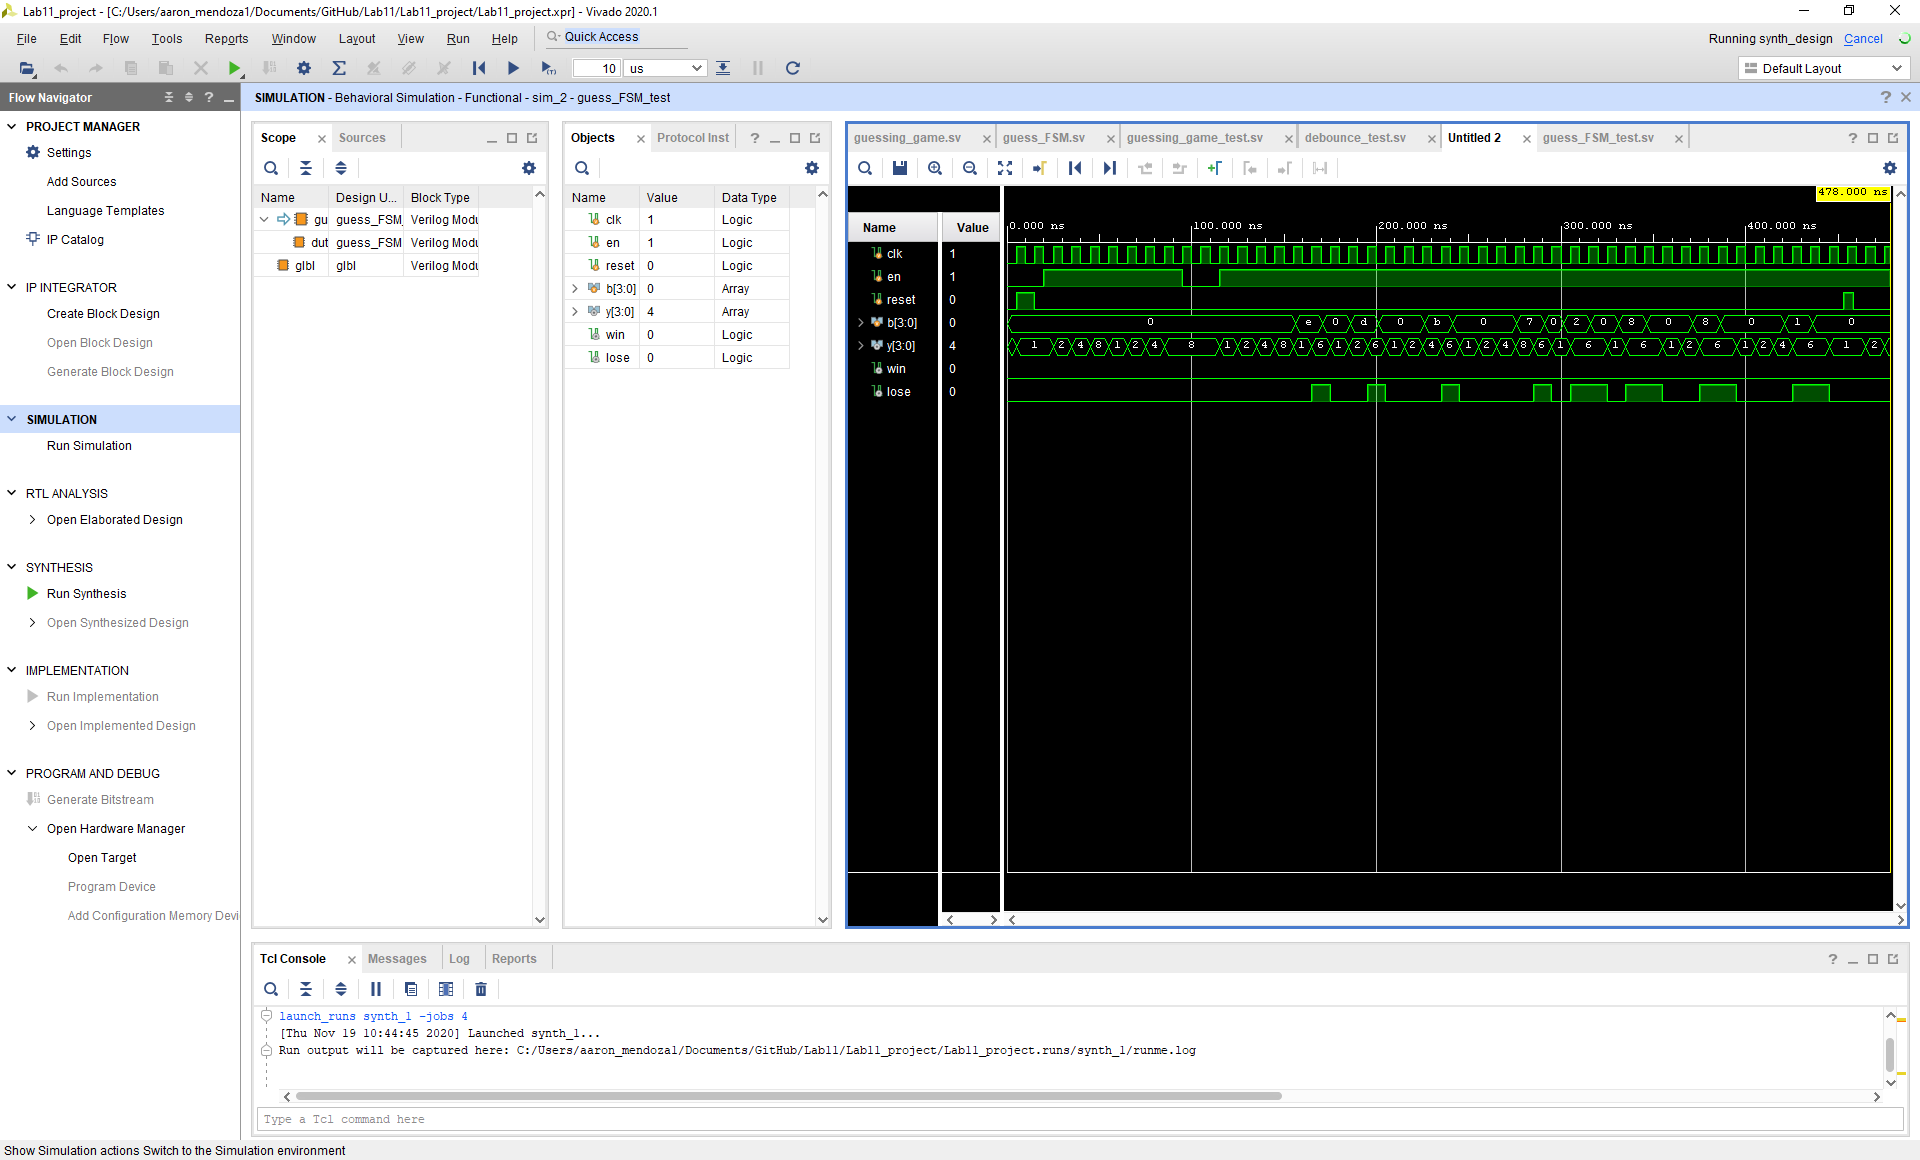
\includegraphics[width=1\textwidth,trim=26cm 18cm 0cm 4.5cm,clip]{guess_FSM_screenshot}
	\caption{Guess-FSM Simulation Screenshot}
	\label{fig:sim_with_table}
\end{figure}

\FloatBarrier

\begin{figure}[ht]\centering
	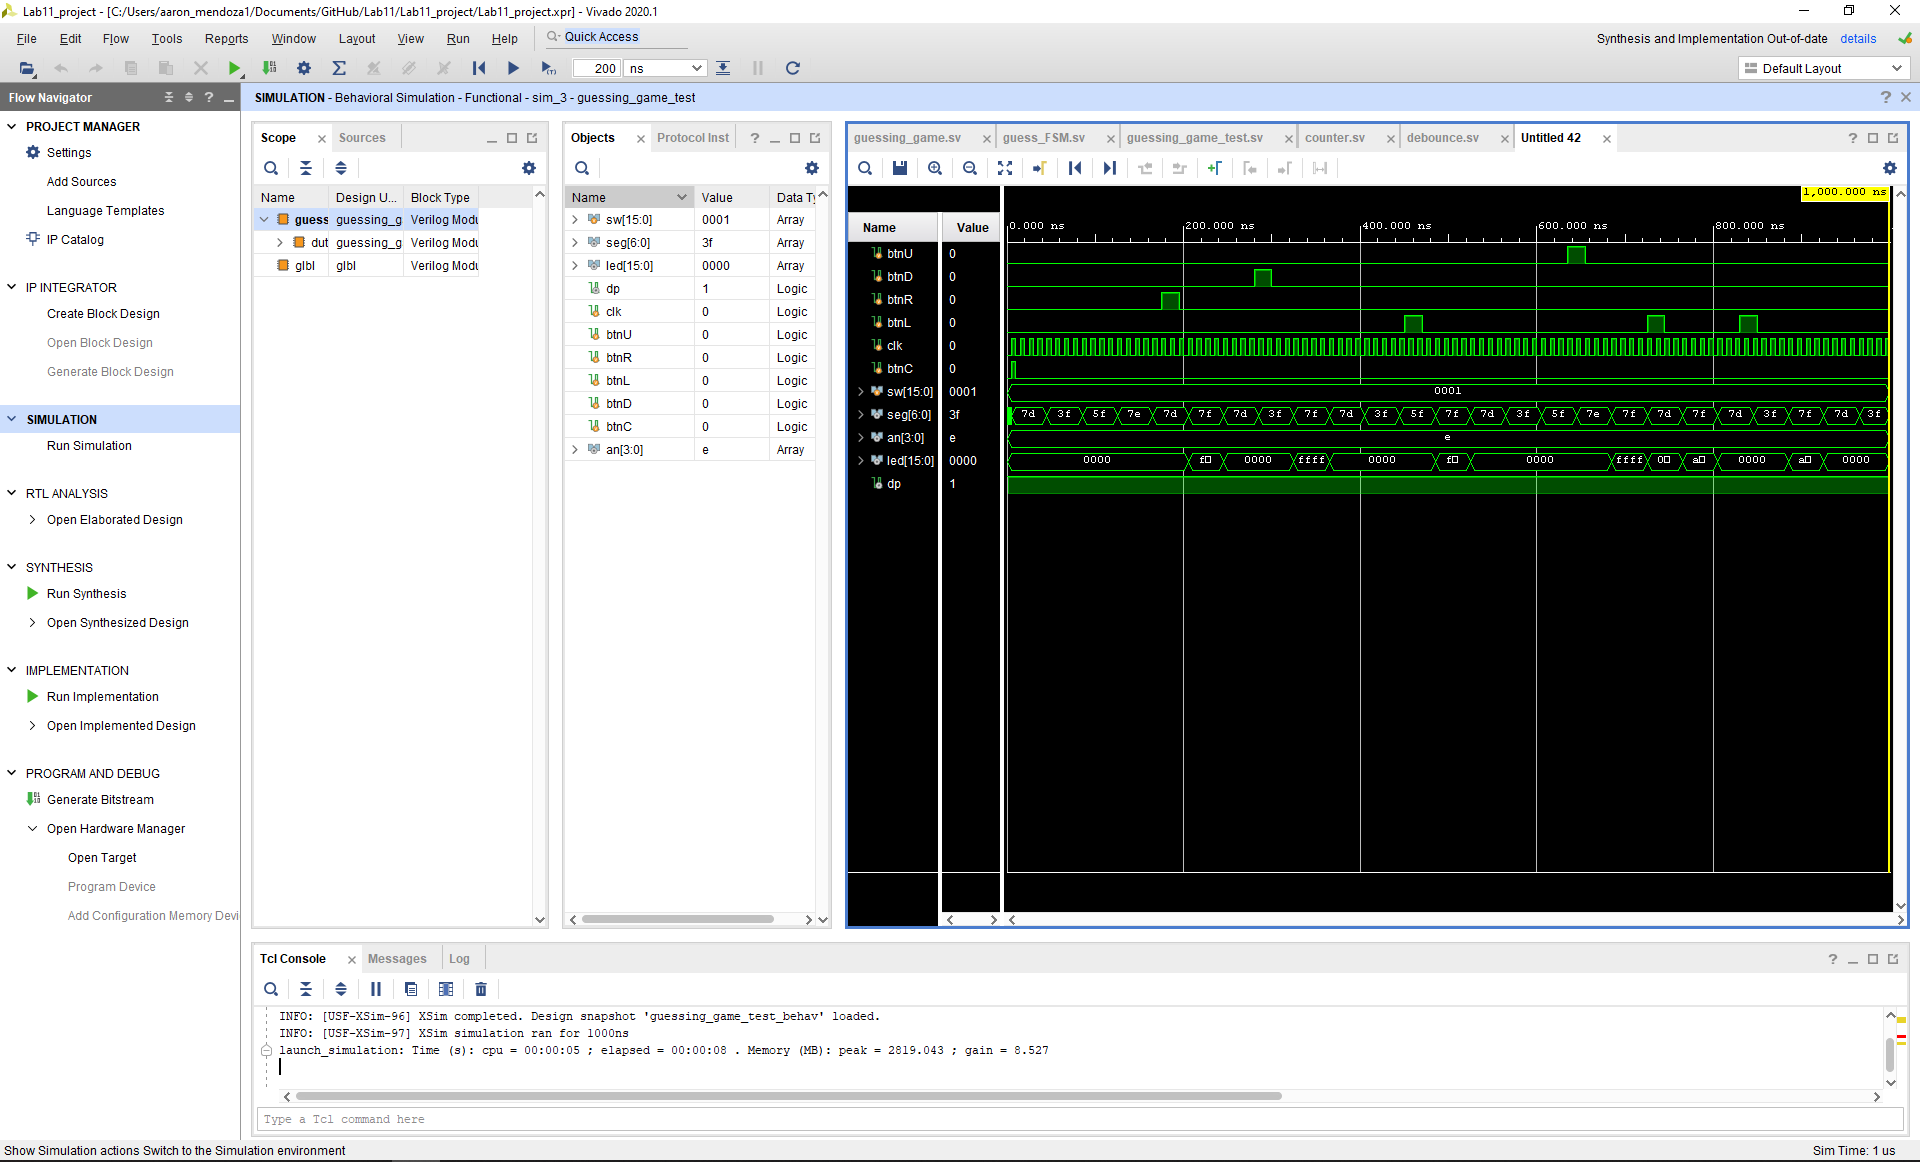
\includegraphics[width=1\textwidth,trim=26cm 15.5cm 0.5cm 4.5cm,clip]{guessing_game_test_screenshot}
	\caption{Guessing Game Simulation Screenshot}
	\label{fig:sim_with_table}
\end{figure}

\FloatBarrier

\begin{table*}[ht]\centering
	\caption{Games Played}
	\label{ALU:tbl:alu_ERT}\medskip
	\begin{tabular}{l|rrrrrrrrrr}
		Game: & 1 & 2 & 3 & 4 & 5 & 6 & 7 & 8 & 9 & 10 \\
		\midrule
		Easy & W & W & W & W & W & W & W & W & W & W \\
		Hard & W & W & W & W & W & W & W & W & W & W \\
		\bottomrule
	\end{tabular}
\end{table*}

\FloatBarrier

The win percentage of both my difficulties was 100 percent. The speed of my moving target was not very fast, but that can easily change by modifying the parameters within my code.

Here is a link to a video that has me playing the game at both difficulties: https://youtu.be/hejE2cdHryo

\section*{Code}

\Verilog[firstline=1, lastline=76, caption=Debounce Module Code]{Lab11_project/codedirectory/debounce.sv}|

\Verilog[firstline=1, lastline=35, caption=Debounce Testbench Code]{Lab11_project/codedirectory/debounce_test.sv}|

\Verilog[firstline=23, lastline=40, caption=Counter Module Code]{Lab11_project/codedirectory/counter.sv}|

\Verilog[firstline=23, lastline=28, caption=MUX Difficulty Module Code]{Lab11_project/codedirectory/mux_diff.sv}|

\Verilog[firstline=23, lastline=120, caption=Guess FSM Module Code]{Lab11_project/codedirectory/guess_FSM.sv}|

\Verilog[firstline=23, lastline=68, caption=Guess FSM Testbench Code]{Lab11_project/codedirectory/guess_FSM_test.sv}|

\Verilog[firstline=23, lastline=109, caption=Guessing Game Module Code]{Lab11_project/codedirectory/guessing_game.sv}|

\Verilog[firstline=23, lastline=63, caption=Guessing Game Testbench Code]{Lab11_project/codedirectory/guessing_game_test.sv}|

\end{document}
